\documentclass[aspectratio=169,10pt]{beamer}
\usepackage{tikz}
\usetikzlibrary{arrows.meta,calc}
\usepackage{graphicx}
\setbeamertemplate{navigation symbols}{}
\setbeamertemplate{footline}{}
\definecolor{ink}{HTML}{122B39}
\definecolor{paper}{HTML}{F5F2E9}
\definecolor{teal}{HTML}{007D80}
\definecolor{mint}{HTML}{5DE2CB}
\definecolor{orange}{HTML}{FFB45B}
\definecolor{muted}{HTML}{B5C9CE}
\definecolor{slate}{HTML}{54717E}
\setbeamercolor{background canvas}{bg=paper}
\newcommand{\txt}[6]{\node[anchor=north west,align=left,text=#4,text width=#3 cm,inner sep=0pt,font=\fontsize{#5}{#6}\selectfont] at (#1,#2)}
\newcommand{\foot}[2]{\txt{0.6}{0.40}{14}{#1}{7}{8}{BIOHACKATHON 2026\quad /\quad MHC PANGENOME\hfill github.com/biohackathon-japan/BH26-asian-hla\qquad #2/3};}
\hyphenpenalty=10000
\begin{document}

\setbeamercolor{background canvas}{bg=ink}
\begin{frame}[plain]
\begin{tikzpicture}[remember picture,overlay,x=1cm,y=1cm,shift={(current page.south west)}]
\txt{0.6}{8.48}{14.8}{mint}{10}{12}{THE BUILD};
\txt{0.6}{7.91}{14.8}{white}{25}{29}{\textbf{Whose HLA is in your reference?}};
\txt{0.6}{6.94}{14.8}{muted}{13}{17}{Five projects. One graph of the MHC, a highly variable immune region.};
\txt{0.6}{5.86}{5.8}{mint}{47}{49}{\textbf{754}};
\txt{0.65}{4.57}{6.3}{white}{16}{19}{MHC haplotypes};
\txt{0.65}{3.72}{6.5}{muted}{8}{10}{\textbf{462 Asian / Arab haplotype entries}\\266 East Asian + 72 South Asian + 124 Arab\\752 donor haplotypes + 2 references};
% Geographic panel and graph topology exported from manuscript Figure 1.
\txt{7.25}{6.22}{8}{muted}{9}{11}{\textbf{Samples by source}};
\node[anchor=north west,inner sep=0] at (7.15,5.79) {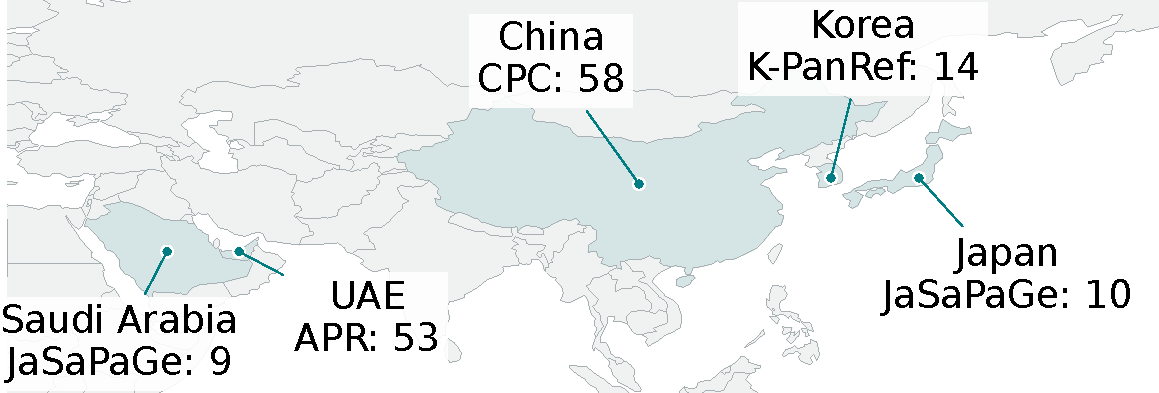
\includegraphics[width=8.0cm,height=2.85cm]{figures/paper-panels/cohort_map.pdf}};
\txt{7.25}{2.82}{8}{white}{9}{11}{HPRC: 232 worldwide; JaSaPaGe: 19 total};
\txt{0.65}{2.58}{6.5}{muted}{8}{10}{376 source sample entries; 371 distinct donors.};
\node[anchor=north west,inner sep=0] at (0.65,2.14) {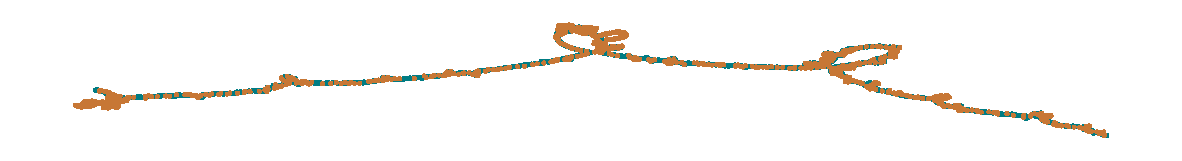
\includegraphics[width=14.7cm,height=1.04cm]{figures/paper-panels/mhc_backbone.pdf}};
\txt{0.65}{1.07}{7.5}{muted}{7}{9}{MHC structural backbone: 1,677 segments, 2,381 links};
\txt{8.5}{1.10}{6.7}{white}{11}{14}{1000 Genomes ($n=2504$)};
\foot{muted}{1}
\end{tikzpicture}
\end{frame}

\setbeamercolor{background canvas}{bg=paper}
\begin{frame}[plain]

\begin{tikzpicture}[remember picture,overlay,x=1cm,y=1cm,shift={(current page.south west)}]
\txt{0.6}{8.48}{14.8}{teal}{10}{12}{THE PAYOFF};
\txt{0.6}{7.91}{14.8}{ink}{24}{28}{\textbf{More haplotypes. Better SV calls.}};
\txt{0.6}{6.93}{14.8}{slate}{12}{16}{79,844 SNV sites and 298 SV-containing graph sites per donor.};
\txt{0.65}{5.96}{9.5}{ink}{12}{15}{\textbf{SV-bearing genotypes recovered exactly (\%)}};
\fill[slate] (0.7,5.25) circle (.07);\txt{0.91}{5.43}{3.7}{slate}{10}{12}{HPRC-only panel};
\fill[teal] (4.6,5.25) circle (.07);\txt{4.81}{5.43}{3.4}{teal}{10}{12}{Expanded panel};
% Scale 65--85%, x = 2.7 + .34 * (accuracy - 65).
\foreach \v in {65,70,75,80,85}{
 \pgfmathsetmacro{\xx}{2.7+.34*(\v-65)}
 \draw[slate!18] (\xx,2.7) -- (\xx,4.75);
 \node[text=slate,font=\small,anchor=north] at (\xx,2.57) {\v};
}
\txt{0.65}{4.41}{2.4}{ink}{10}{14}{East Asian\\20 donors};
\txt{0.65}{3.36}{2.4}{ink}{10}{14}{South Asian\\20 donors};
\draw[teal!40,line width=5pt] (5.199,4.05) -- (6.525,4.05);
\draw[teal!40,line width=5pt] (6.212,3.0) -- (6.882,3.0);
\foreach \x/\y/\val/\col/\labelx in {5.199/4.05/72.4/slate/5.199,6.525/4.05/76.2/teal/6.525,6.212/3.0/75.3/slate/6.05,6.882/3.0/77.3/teal/7.04}{
 \fill[\col] (\x,\y) circle (.095);
 \node[text=\col,font=\bfseries\small,anchor=south] at (\labelx,\y+.15) {\val};
}
\fill[ink,rounded corners=5pt] (10.2,2.62) rectangle (15.35,5.83);
\txt{10.57}{5.54}{4.5}{mint}{34}{37}{\textbf{+3.9}};
\txt{10.57}{4.52}{4.45}{white}{10}{13}{points in East Asian donors};
\txt{10.57}{3.95}{4.45}{muted}{9}{12}{95\% CI: +2.4 to +5.3};
\txt{10.57}{3.40}{4.45}{muted}{9}{12}{South Asian: +2.0 points\\95\% CI: +0.3 to +3.5};
\txt{0.65}{1.99}{14.7}{ink}{14}{18}{\textbf{SV-bearing truth genotypes: 1,465 EAS + 1,577 SAS.}};
\txt{0.65}{1.20}{14.7}{slate}{8}{11}{Shared-SNV comparison: 1,007,636 genotype comparisons per ancestry group.\\40-donor pilot; assembly truth. Test families excluded from panels; test assemblies remain in graph topology.};
\foot{slate}{2}
\end{tikzpicture}
\end{frame}

\setbeamercolor{background canvas}{bg=ink}
\begin{frame}[plain]
\begin{tikzpicture}[remember picture,overlay,x=1cm,y=1cm,shift={(current page.south west)}]
\txt{0.6}{8.48}{14.8}{mint}{10}{12}{THE TYPER};
\txt{0.6}{7.91}{14.8}{white}{25}{29}{\textbf{DogoHLA}};
\txt{0.6}{6.94}{14.8}{muted}{14}{18}{A pangenome-native, population-specific HLA typer.};
% Population-specific sequences enter read collection and structural inference.
\foreach \x/\heading/\detail in {0.65/{Collect reads}/{AsianPGR haplotypes},4.45/{Call and phase}/{Read-backed variants},8.25/{Reconstruct}/{Graph-supported indels},12.05/{Type HLA}/{Sequences + HLA names}}{
 \fill[white,opacity=.07,rounded corners=3pt] (\x,5.11) rectangle +(3.15,1.11);
 \txt{\x+.12}{6.05}{2.92}{mint}{11}{13}{\textbf{\heading}};
 \txt{\x+.12}{5.62}{2.92}{white}{8}{10}{\detail};
}
\foreach \x in {3.97,7.77,11.57}{\draw[-{Latex[length=2mm]},muted,line width=.8pt] (\x,5.65)--+(0.35,0);}
\txt{0.65}{4.84}{14.7}{muted}{8}{10}{Uses SpecHLA components for alignment and small variants; panel graphs supply supported noncoding changes.};
\txt{0.65}{4.28}{8.5}{white}{12}{15}{\textbf{Preliminary: exact whole-gene sequences}};
\txt{0.65}{3.77}{8.5}{muted}{9}{12}{8 development donors $\times$ 8 genes $\times$ 2 haplotypes};
\txt{0.65}{3.17}{3.6}{muted}{11}{14}{Native SpecHLA};
\fill[slate!40!ink] (4.00,2.68) rectangle (8.7,3.02);
\fill[muted] (4.00,2.68) rectangle (5.321875,3.02);
\txt{7.4}{3.47}{1.4}{white}{14}{16}{36/128};
\txt{0.65}{2.37}{3.6}{mint}{11}{14}{DogoHLA};
\fill[slate!40!ink] (4.00,1.88) rectangle (8.7,2.22);
\fill[mint] (4.00,1.88) rectangle (6.092969,2.22);
\txt{7.4}{2.67}{1.4}{mint}{14}{16}{57/128};
\fill[white,rounded corners=4pt] (9.45,1.90) rectangle (15.35,4.32);
\txt{9.65}{4.18}{5.4}{ink}{8}{10}{\textbf{AsianPGR class II / DRB structure}};
\node[anchor=north west,inner sep=0] at (9.66,3.83) {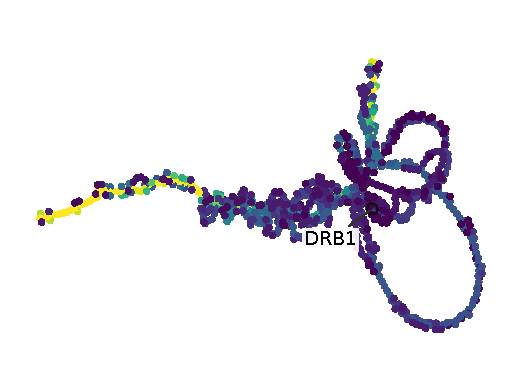
\includegraphics[width=5.35cm,height=1.62cm]{figures/paper-panels/classII_drb.pdf}};
\txt{9.66}{2.13}{5.4}{slate}{6.5}{8}{Reference illustration; colour = haplotype sharing.};
\txt{0.65}{1.58}{14.7}{white}{10}{12}{22.8\% fewer sequence edits; correct two-field genotypes: 61/63 $\rightarrow$ 62/63.};
\txt{0.65}{1.13}{14.7}{orange}{11}{14}{\textbf{Selected development results; further independent analysis is needed.}};
\txt{0.65}{0.72}{14.7}{muted}{7}{9}{Global whole-gene matches to assembly truth; larger independent evaluation ongoing.};
\foot{muted}{3}
\end{tikzpicture}
\end{frame}
\end{document}
